<<<<<<< HEAD
\section{Command-Muster}

\subsection{Problemstellung}
Es soll eine Universalfernbedienung entworfen werden. Hierbei k"onnen verschiedene Haushaltsger"ate angeschlossen werden. Die Fernbedienung soll f"ur jedes angeschlossene Ger"at einen An- und Ausschalter zur Verf"ugung stellen. Problem hierbei. Diverse Ger"atschaften besitzen haben unterschiedliche Schnittstellen. Bei manchen hei"sen diese schlicht und ergreifend anders als gefordert, bei anderen gibt es eine derart schlichte Kontrollfunktion nicht. Ein Beispiel w"are hier zum Beispiel ein Garagentor welches auf und zu gemacht werden kann aber auch eine Stereoanlage soll nicht nur angeschaltet werden, es soll auch ein Lied mit einer bestimmten Lautst"arke gespielt werden. 

Au"serdem soll es m"oglich sein eine gerade angefragte Aktion r"uckg"angig zu machen. 

\begin{figure}[b!]
	\centering
	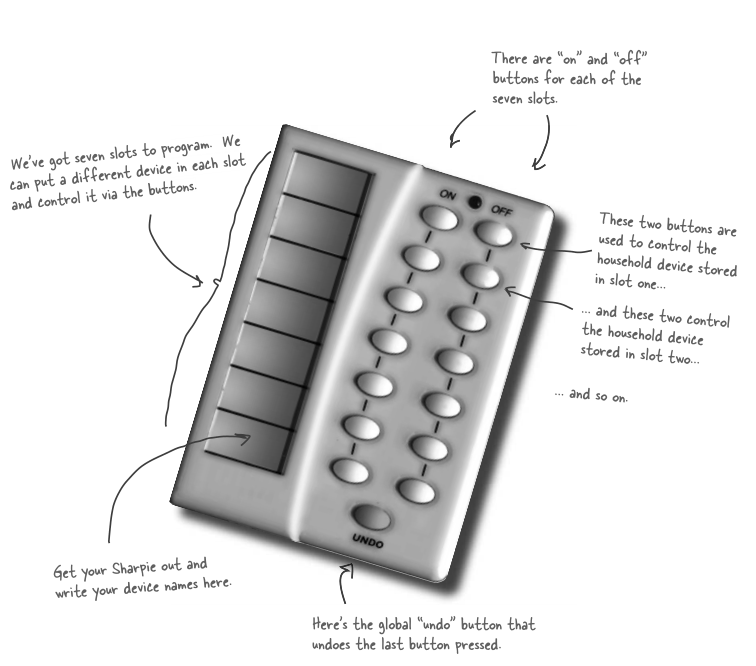
\includegraphics[width=.6\linewidth]{command/img/commandPatternRemote}
	\caption{UML-Darstellung der zu implementierenden Fernsteuerung}
	\label{fig:commandRemote}
\end{figure}

\paragraph{L"osung}
Anfragen werden per Schnittstelle gekapselt. Jede Art von Ger"at API welche an die Fernbedienung angeschlossen werden soll muss von einer Klasse welche das Command-Interface f"ur eine Art von Ger"at aufgenommen werden k"onnen. Diese Command-Klasse birgt allerdings nur die Methode(n) zum tats"achlichen Ausf"uhren der Kommandos. Diese Methode kann anschlie"send von der eigentlichen Fernbedienung aufgerufen werden. Eine Fernbedienung besitzt nun irgendeine Art von Collection um diversen Slots die gerade beschriebenen Kommando-Objekte zuweisen zu k"onnen. 

Um Slots zu sperren welche keine Belegung besitzen kann man entweder eine Pr"ufung auf die Nullreferenz einbauen oder ein Default-Kommando implementieren was nichts tut und somit auch keine Nullpointerexception ausl"ost. 

\paragraph{Undo-Fkt.} 
Die einfachste Art dies umzusetzen ist jeweils zwei getrennt Command-Objekt f"ur das An-/Ausschalten von Ger"aten zu implementieren. Wenn man nun in der Fernbedienung eine Instanzvariable mit dem jeweils zuletzt ausgef"uhrten Befehl setzt. Damit ein Aufruf von undo funktionieren kann muss die Commandschnittstelle jeweils diese Funktion implementieren. Um mehrere Undo's hintereinander auszuf"uhren reicht ein rekursiver Aufruf, da die \emph{gemerkte} Instanzvariable selbst ein Command-Objekt ist und somit ebenfalls einen Verlauf besitzt.  


\subsection{Erkl"arung des Musters}
\paragraph{Definition}
Das Command-Muster kapselt eine Anfrage als ein Objekt, dies erm"oglicht polymorphes Verhalten mit unterschiedlichen Anfragen, Warteschlangen oder Log-Anfragen. Mit diesem Muster wird au"serdem eine Undo-Option erm"oglicht.

\paragraph{Beschreibung}
Ein Command-Objekt kapselt einzelne Anfragen indem ein Interface nach spezifischen Gruppen implementiert wird. Dieses Interface bietet eine wie bereits erw"ahnt eine Methode \emph{execute}. Diese Methode arbeitet mit einer im Konstruktor "ubergebenen Instanzvariable. Da es eine klare Trennung zwischen dem Erstellen der Command-Objekte und dem Ausf"uhren gibt, gibt es hierbei viele Freiheiten. Es ist bspw. m"oglich erst mehrere Befehle zu sammeln bevor sie nacheinander (oder gar gleichzeitig) ausgef"uhrt werden (siehe Meta Command Muster).

\begin{figure}[b!]
	\centering
	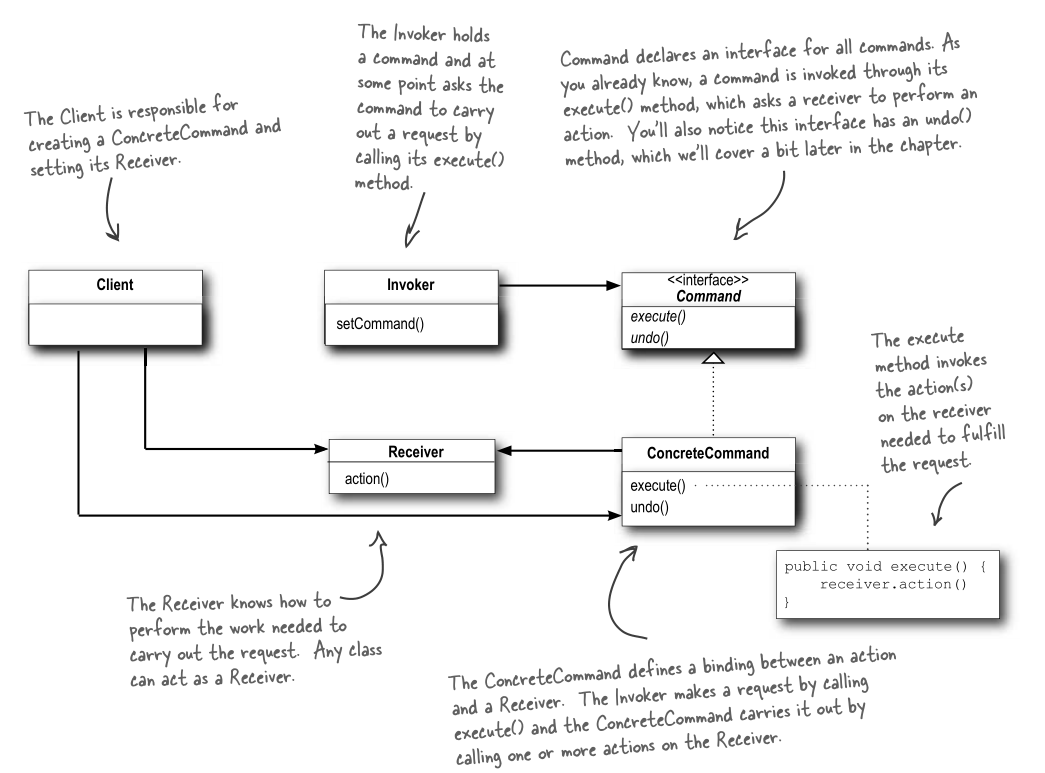
\includegraphics[width=1\linewidth]{command/img/commandUML}
	\caption{UML-Darstellung der zu implementierenden Fernsteuerung}
	\label{fig:commandUML}
\end{figure}

\paragraph{Macro-Commands}
Um mehrere Command-Objekte "uber einen Slot in der Fernbedienung auszuf"uhre, wird kann man einfach eine Instanzvariable mit einer Collection von Commando-Objekten welche ausgef"uhrt werden sollen implementieren. In der \emph{execute}-Methode werden diese dann alle nacheinander ausgef"uhrt. 

\begin{figure}[b!]
	\centering
	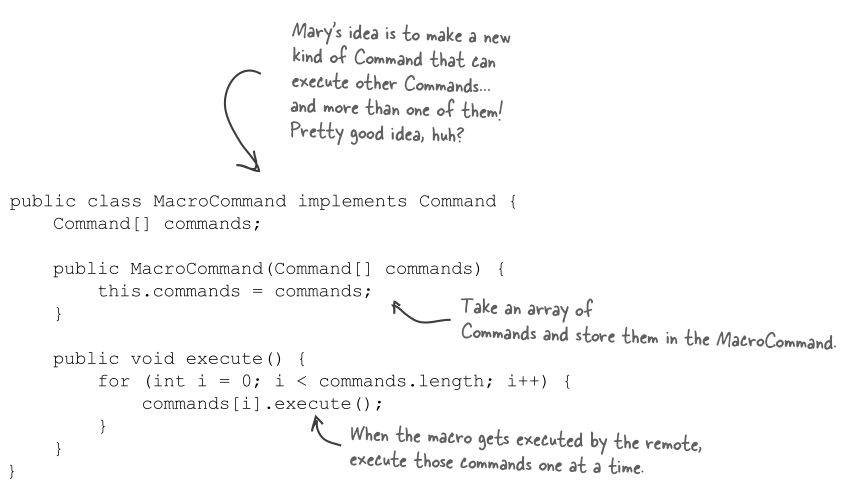
\includegraphics[width=1\linewidth]{command/img/macroCommandCodeExample}
	\caption{Codetemplate des Macro-Command-Musters}
	\label{fig:macroCommand}
\end{figure}


\subsection{Vorteile}
\begin{itemize}
	\item Die Bearbeitung der Aufgaben ist komplett gekapselt
	\item Ideal f"ur parallele Verarbeitung
	\item Einfach Erweiterbar, z.B. Queue welche von mehreren Threads abgearbeitet wird. 
	\item M"oglich einfach logging und load Methode in die Schnittstelle aufzunehmen. Dies erm"oglicht es im Fehlerfall einen Datenverlust zu vehindern. 
\end{itemize}
=======
\section{Command-Muster}

\subsection{Problemstellung}
Es soll eine Universalfernbedienung entworfen werden. Hierbei k"onnen verschiedene Haushaltsger"ate angeschlossen werden. Die Fernbedienung soll f"ur jedes angeschlossene Ger"at einen An- und Ausschalter zur Verf"ugung stellen. Problem hierbei. Diverse Ger"atschaften besitzen haben unterschiedliche Schnittstellen. Bei manchen hei"sen diese schlicht und ergreifend anders als gefordert, bei anderen gibt es eine derart schlichte Kontrollfunktion nicht. Ein Beispiel w"are hier zum Beispiel ein Garagentor welches auf und zu gemacht werden kann aber auch eine Stereoanlage soll nicht nur angeschaltet werden, es soll auch ein Lied mit einer bestimmten Lautst"arke gespielt werden. 


\begin{figure}
	\centering
	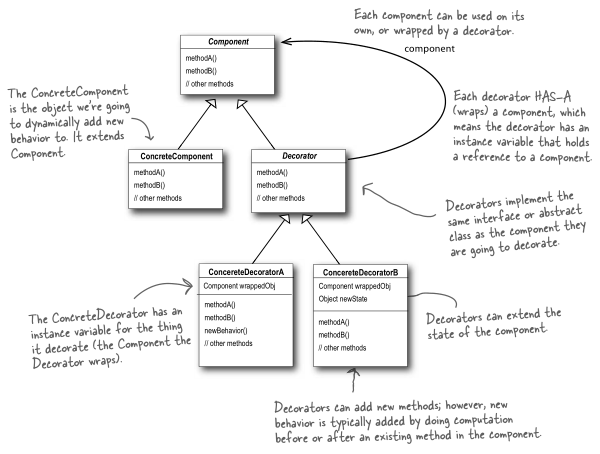
\includegraphics{decorator/img/decoratorUML}
	\caption{UML-Darstellung der zu implementierenden Fernsteuerung}
	\label{fig:commandRemote}
\end{figure}
>>>>>>> 7385d687a6c25fd8f0ca4aec01f29fe339feb8b3
